%!TEX root = Bericht.tex
\graphicspath{{graphics/HMI/}{graphics/control_modes/}}
\chapter{Finding a Hardware and Software Solution}
\label{cha:findHardSoftSolution}
In the following it is described how the the previously defined control modes were realized and what else lead to the finally realized HMI, described in the last section \ref{sec:realization}. On the one hand there was the hardware which had to be chosen and on the other the software to realize the control modes with that hardware had to be written.



\section{Requirements}
\label{sec:requirements}
One of the goals of this Bachelor's Thesis was to develop a HMI which was tailored to \textsc{Skye}. In the following listing, all requirements demanded for such a HMI are pointed out: \\

The hardware used should...
\begin{itemize}
\item{offer intuitive control for six DOF, i.e. fit the defined control modes, }
\item{be portable,}
\item{offer wireless connection, i.e. ports for attaching a \textsc{XBee} module and a Wifi router,}
\item{be able to display the live view of \textsc{Skye},}
\item{offer the possibility to set waypoints for \textsc{Skye},}
\end{itemize}
whereas the used operation system should be compatible with the driver of the \textsc{XBee} module and with ROS\footnote{The decision to use a \textsc{XBee} module and Wifi for communication is explained in \cite{burri}. There, it is also explained how \textsc{ROS} was needed to process imagery.}.


\section{Existing Solutions}
\label{sec:existingSolutions}
Existing HMI solutions were analyzed in order to find out, whether they would be convenient to adopt or whether they would fulfill the requirements on their own. 


\subsection{Hardware}
\label{sub:hardware}

Figure \ref{fig:devices taken into consideration} shows all devices which were taken into closer consideration. The gamepad option was drapped as it would offer the same possibilities as RC does with the drawback of not being a stand alone device. Smartphones could not be used as they run with a operation systems not compatible with \textsc{ROS}\footnote{This held true when this Thesis was written and might be different nowadays as almost everything.}.

\begin{figure}[h]		
	\small{
		\begin{center}
			\parbox[b]{0.25\textwidth}{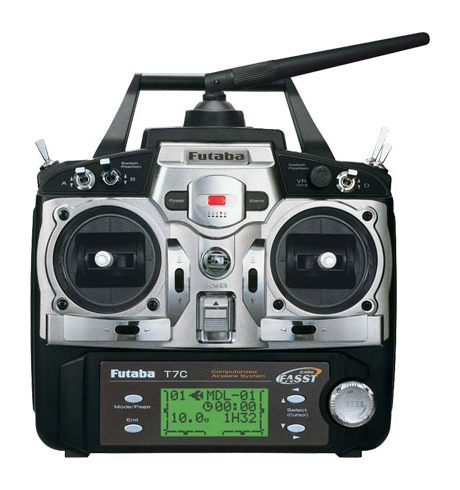
\includegraphics[width=0.23\textwidth]{futaba_7C_radio}
			\begin{center}RC \end{center}}
			\hspace{0.05\textwidth}
			\parbox[b]{0.25\textwidth}{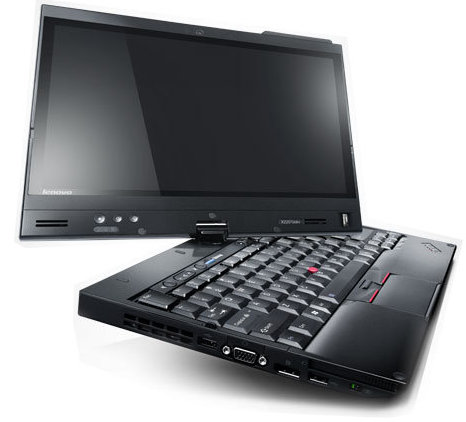
\includegraphics[width=0.25\textwidth]{x220t_hero}
			\begin{center}Tablet \end{center}}
			\hspace{0.05 \textwidth}
			\parbox[b]{0.25\textwidth}{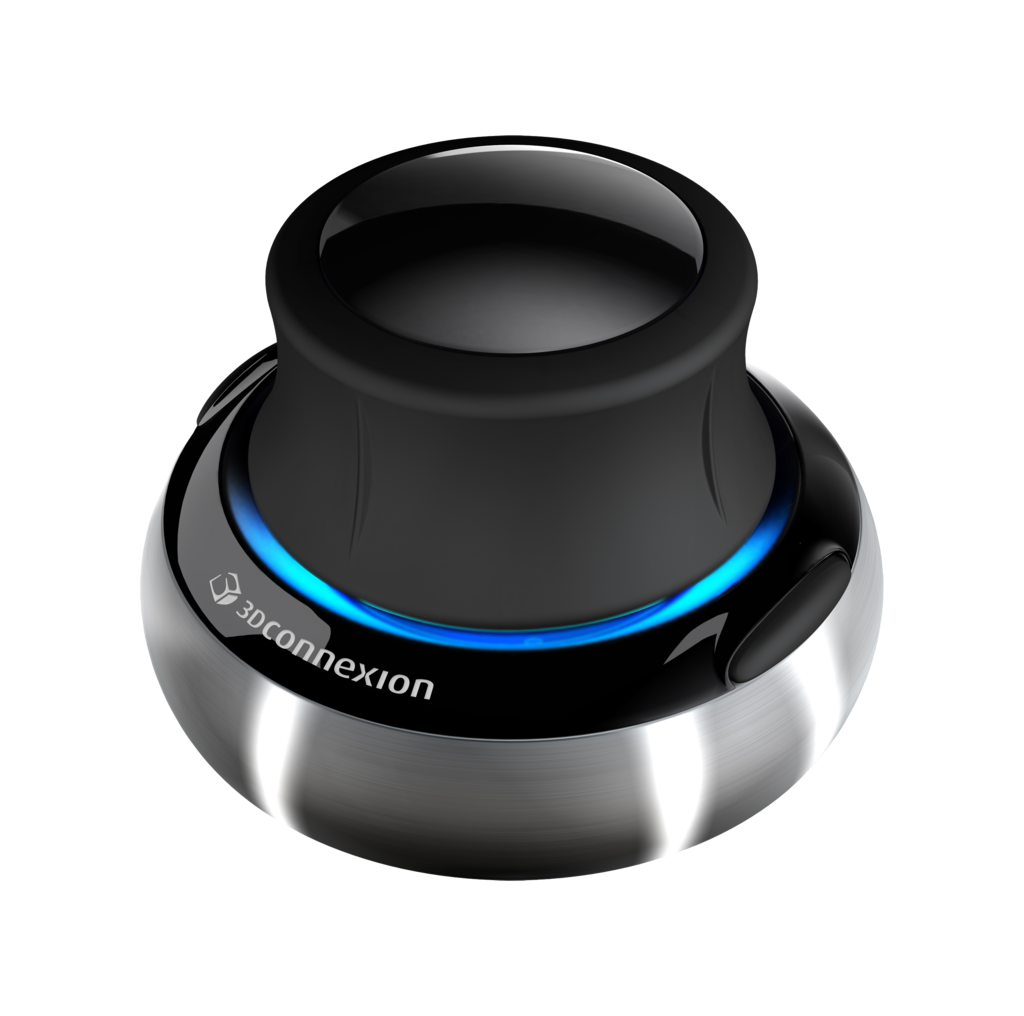
\includegraphics[width=0.25\textwidth]{3dx_productimage}
			\begin{center}3D Mouse \end{center}}			
			\vspace{0.005\textwidth}
			\hspace{0.05\textwidth}			
			\parbox[b]{0.25\textwidth}{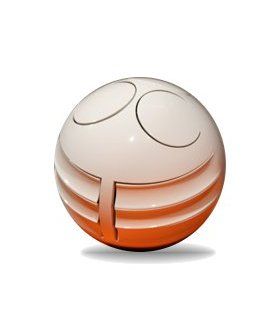
\includegraphics[width=0.25\textwidth]{qgo_sphere_cut}
			\begin{center}Qgo Sphere \end{center}}
			\hspace{0.05\textwidth}
			\parbox[b]{0.25\textwidth}{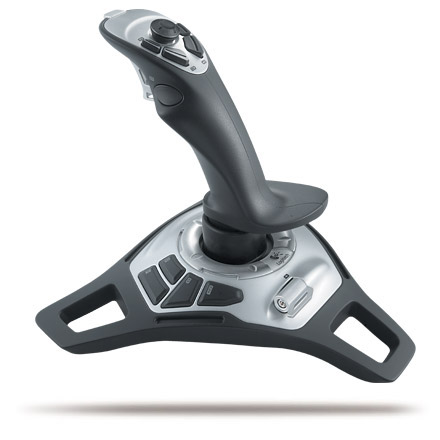
\includegraphics[width=0.25\textwidth]{Logitech-Freedom-Cordless-Joystick}
			\begin{center}Joystick \end{center}}
			\caption[Different devices taken into consideration]{Different devices taken into consideration}
			\label{fig:devices taken into consideration}	
		\end{center}
	}			
	\vspace{4.5mm}
\end{figure}

Table \ref{tab:requirements and expectations for hardware} shows the rating of the considered devices. It is visible that a solution in combination with a tablet had to be used, as only a tablet is able to fulfill certain criteria and to run \textsc{ROS}. Although the Qgo Sphere \footnote{In  \cite{kammermann} the usage of the Qgo Sphere as an input device for a ballbot is discussed.} would be most intuitive to use with \textsc{Skye}, a 3D mouse, i.e. a space navigator from \textsc{3DConnection}, was chosen as a supplementary device to the tablet. Because of the fix-installed infrared sensors needed for the detection of the sphere's translational movements, the Qgo Sphere is not portable, which made it inconvenient to use for \textsc{Skye}. For the tablet a \textsc{Lenovo} X220 was chosen whereas a \textsc{Futuba} 7C RC was chosen as a backup in case of a tablet failure.


\begin{table}[H]		% [H] indicates that the table should be right here.
	%\begin{tabularx}{\textwidth}{p{0.125\textwidth}p{0.2\textwidth}|p{0.06\textwidth}p{0.075\textwidth}p{0.08\textwidth}p{0.1\textwidth}p{0.08\textwidth}}	% add p{size_of_colomn} for every new column you'd like to have. If you put a | between the p then there is a vertical line between the columns. 
	\begin{center}
 \begin{tabular}{ll|ccccc}
\multicolumn{2}{l|}{Device}	& \rotatebox{90}{\mbox{RC}} 	& \rotatebox{90}{\mbox{Tablet}} 	&\rotatebox{90}{\mbox{3D Mouse}}	&\rotatebox{90}{\mbox{Qgo Sphere}}	&\rotatebox{90}{\mbox{Joystick}}  \\
	\toprule[1.25pt]				%define the line thickness of the top rule
	\multicolumn{2}{l|}{Stand alone}							&\checkmark		&\checkmark		&-			&-			&-\\
	\hline%\midrule
	\multirow{5}{*}{Matching}		&Test Phase					&-				&\checkmark		&-			&-			&-\\
									&Direct Control				&\checkmark		&\checkmark		&\checkmark	&\checkmark	&\checkmark\\
									&Assisted Control			&\checkmark		&\checkmark		&\checkmark	&\checkmark	&\checkmark\\
									&Half Automatic Control		&-				&\checkmark		&-			&-			&- \\
									&Full Automatic Control		&-				&\checkmark		&-			&-			&-\\
	
	\hline%\midrule
	\multicolumn{2}{l|}{Live View}							&-				&\checkmark		&-			&-			&-\\
	\hline%\midrule
	\multicolumn{2}{l|}{Intuitive}								&quite	&quite	&very&most&quite\\
	\hline%\midrule
	\multicolumn{2}{l|}{Portable}								&most	&quite	&quite&not &quite\\
		
	\bottomrule[1.25pt]
	%\end{tabularx} 
	\end{tabular}
	\caption[Requirements and Expectations for the Hardware]{Requirements and Expectations for the Hardware}
	\label{tab:requirements and expectations for hardware}
	\end{center}
\end{table}


\subsection{Software}
\textit{QGroundControl, OpenPilot, Qt-Libraries}
\textsc{Google} and \textsc{Apple} showed how intuitive a software could be in combination with a  touchscreen with their operating systems for smartphones. They offer the user unknown flexibility in adopting the GUI to his needs. However, out of \textsc{Windows}, \textsc{Ubuntu}, \textsc{Mac OS}, \textsc{iOS} and \textsc{Android}, \textsc{Ubuntu} was the only operating system which provided complete support for \textsc{ROS}  Therefore \textsc{Ubuntu 11.10} was chosen as the operating system for the tablet.\\
As it was clear that there was no GUI ready to use unchanged for the HMI, open source software was analyzed in order to adopt it for \textsc{Skye}. Using \textsc{QGroundControl} (described in section \ref{subsec:qGroundControl}) was the best option. On the one hand it already offered the commonly used tools to control a UAV, and on the other hand a good support in adopting it to the needs of \textsc{Skye} was granted as it was also developed at the \textsc{ETH}.




\section{Realization}
\label{sec:realization}



\subsection{Compact and Convenient Solution}
\textit{About advantages of TabletPC, 3dMouse, RC}
Using a 3D mouse, connected to a tablet computer has a lot of advantages. Both devices can be put on a board with suspenders. Like the pilot has a compact, portable control unit, without any external hardware interconnected, (Compare figure \ref{fig:HMI_in_Action}). While the 3D mouse provides intuitive control of the 6DOF, the tablet with its GUI is used to filter and route the signals of the 3D Mouse or serves as a highly modular touch input device on its own. With \textsc{QGroundControl} running on it, It also enables the pilot to adjust the controller and to set waypoints, while during the whole flight the live view of \textsc{Skye} is displayed. (More on that in section \ref{subsec:qGroundControl}) In case the tablet should crash, the RC can be used to bring down \textsc{Skye} safely.

\begin{figure}[H]
	\begin{center}
		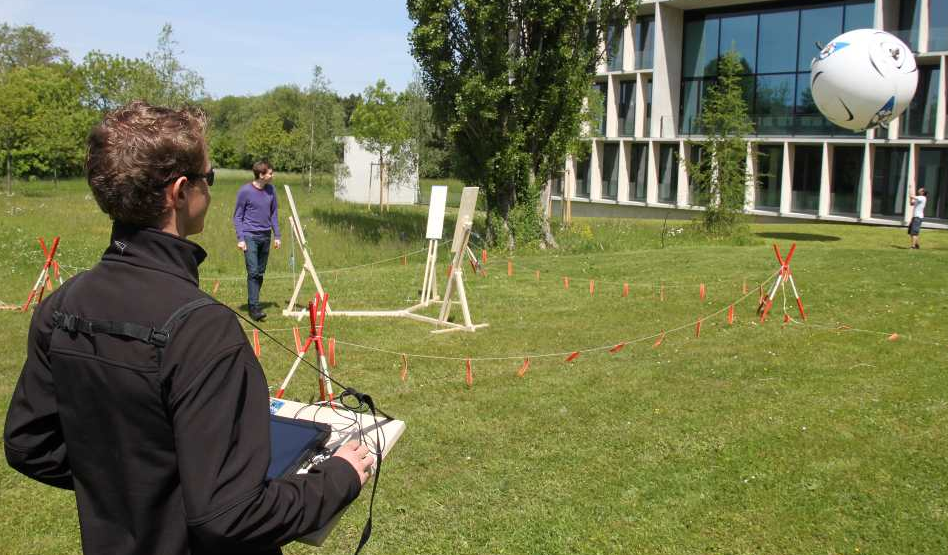
\includegraphics[width=0.85\textwidth]{graphics/HMI_in_Action}
		\caption{The compact, portable control unit in action}  
		\label{fig:HMI_in_Action}
	\end{center}
\end{figure}



\subsection{QGroundControl}
\label{subsec:qGroundControl}
\textit{Adaptions in QGroundControl, 3dMouse, Touchscreen, Splines and Trajectory Controller \\ Only how it looks like and how to use. All ``important'' widgets are shown in detail. Implementation of 3dMouse and Touchscreen are not described further.picture of touch in action, mail final presentation}


\begin{figure}[H] % [H] steht dafür, dass das Bild genau hier im Text sein soll.
	\begin{center}
		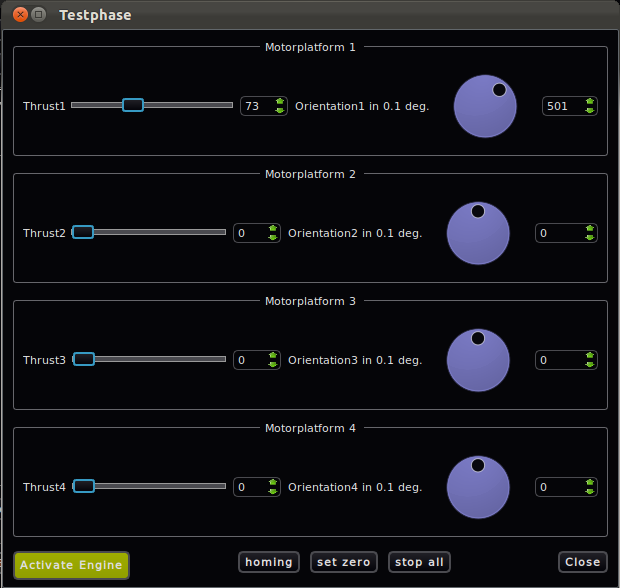
\includegraphics[width=0.7\textwidth]{qgc_test_phase}
		\caption[Test Phase realization]{The \textit{Test Phase} widget allows to adjust each actuation input separately. The input for the four thrusters is set by sliders and the orientation is set by turning the knobs. There is a main button (Activate Engine) to start and stop the motors.}  
		\label{figure:qgc_test_phase}
	\end{center}
\end{figure}

\begin{figure}[H] % [H] steht dafür, dass das Bild genau hier im Text sein soll.
	\begin{center}
		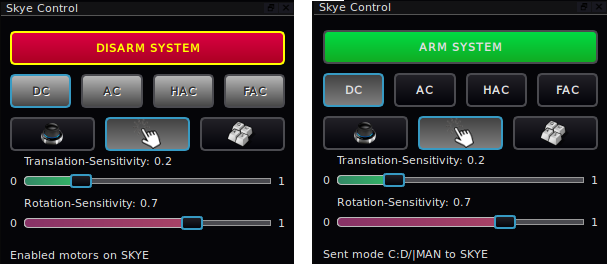
\includegraphics[width=0.6\textwidth]{qgc_skye_control}
		\caption[Main control widget]{On the main control widget, the control mode (Direct Control (DC), Assisted Control (AC), Half Automatic Control (HAC), Full Automatic Control (FAC)) can be set. The colored arm/disarm button is used to (de-)activate the actuators. The input mode (3D Mouse, Touchscreen, Keyboard) can be set by three buttons. The two sliders allow to adjust the input scaling. Indoor flights need usually smaller but more accurate inputs, while outdoors more power is needed.}  
		\label{figure:qgc_skye_control}		
	\end{center}
\end{figure}

\begin{figure}[H] % [H] steht dafür, dass das Bild genau hier im Text sein soll.
	\begin{center}
		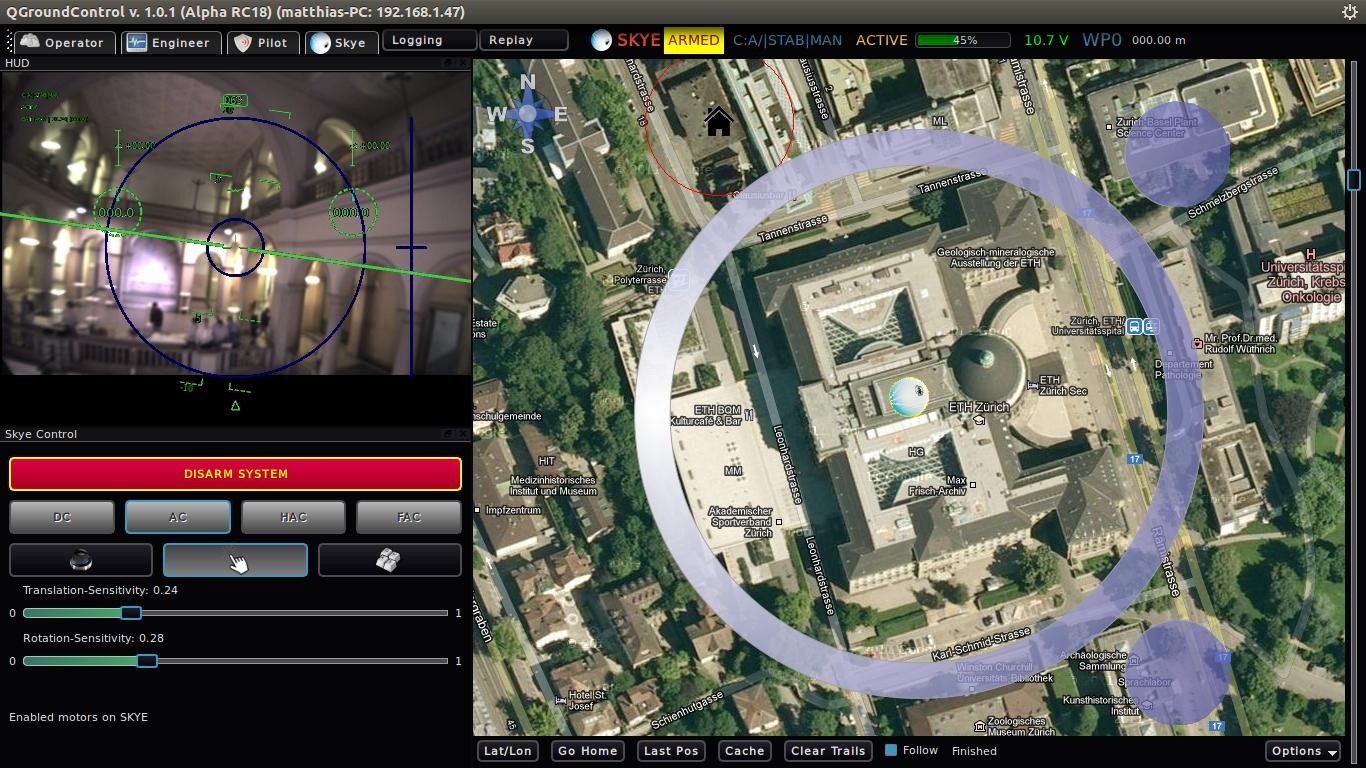
\includegraphics[width=0.8\textwidth]{qgc_manual_control}
		\caption[Manual control view of Graphical User Interface]{The pilots view on the GUI\footnotemark : The HUD shows the video stream and enables rotational touch inputs. The map widget shows the position of \textsc{Skye} and allows to set translational inputs. Note that in a first approach these inputs are always given in the camera frame and not as might expected in inertial frame. Further testing will show which mode is more intuitive. The GUI also includes the main control widget.}  
		\label{figure:qgc_manual_control}		
	\end{center}
\end{figure}
\footnotetext{This screenshot is a reproduced situation of the flight in ETH main building. Obviously, no GPS information were available then.}

\begin{figure}[H] % [H] steht dafür, dass das Bild genau hier im Text sein soll.
	\begin{center}
		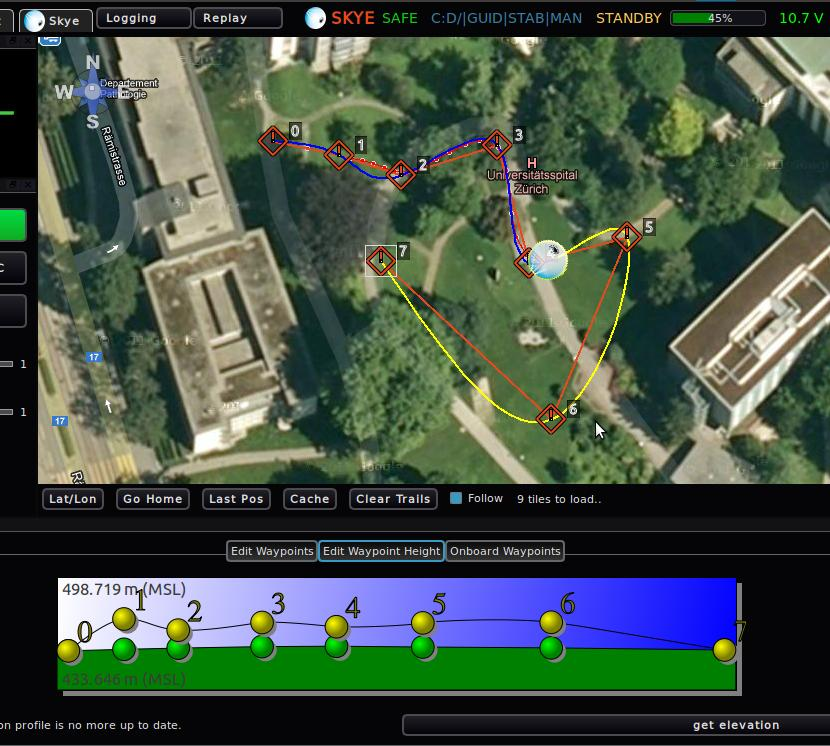
\includegraphics[width=0.8\textwidth]{qgc_automatic_control}
		\caption[Automatic control view of Graphical User Interface]{The user can set waypoints on Google Maps. Spline curves are calculated based on these nodes (yellow line). The part of the path that is already reached is displayed in blue. In the lower part, the height of the waypoints  can be set (yellow points). The actual height of the ground at the waypoints position is also provided by the Google Elevation API\footnotemark (green points and shape). In a further step, the trajectory controlling will be adapted to the real system.}  
		\label{figure:qgc_automatic_control}		
	\end{center}
\end{figure}
\footnotetext{\url{https://developers.google.com/maps/documentation/elevation/}}


\subsection{Mavlink}
\textit{Summary of Protocal, adaptions and use for} \textsc{Skye}